\makesubsectionpage{Naiver Bayes}


\begin{frame}{Naive-Bayes-Klassifikator: Grundidee}
\begin{columns}
\column{0.58\textwidth}
Der \textbf{Naive-Bayes-Klassifikator} ist ein einfaches, aber oft
erstaunlich leistungsfähiges Verfahren auf Basis der
\textbf{Wahrscheinlichkeitsrechnung}.

\vspace{0.4em}
\begin{itemize}
  \item Grundlage ist der \textbf{Satz von Bayes}.
  \item Gesucht: die \textbf{wahrscheinlichste Klasse} für einen gegebenen
        Merkmalsvektor.
  \item \textbf{„Naiv":} alle Merkmale werden als \textbf{voneinander
        unabhängig} angenommen.
\end{itemize}

\vspace{0.4em}
{\footnotesize\itshape Diese Vereinfachung stimmt selten exakt -- in der
Praxis funktioniert sie aber oft sehr gut.}

\column{0.38\textwidth}
\begin{blockC1}{Satz von Bayes}
\centering
\vspace{0.2em}
\[
  P(K \mid M) = \frac{P(M \mid K)\, P(K)}{P(M)}
\]
\vspace{0.2em}

{\footnotesize $K$: Klasse, $M$: Merkmale}
\end{blockC1}
\end{columns}
\end{frame}


\begin{frame}{Satz von Bayes: anschaulich am Beispiel}
\begin{columns}
\column{0.52\textwidth}
\footnotesize
\textbf{100 Studierende.} 60 lernen, 40 nicht. Wer lernt, besteht zu 90\,\%,
wer nicht lernt zu 30\,\%.

\vspace{0.4em}
\centering
\resizebox{\linewidth}{!}{%
\begin{tikzpicture}[
  knoten/.style={circle, draw=PrimaryColor, very thick, minimum size=6mm,
                 font=\scriptsize},
  blatt/.style={rounded corners=3pt, draw, very thick, font=\scriptsize,
                inner sep=3pt, text width=1.6cm, align=center, minimum height=1.1cm},
  kante/.style={->, >=Stealth, thick},
  lab/.style={font=\scriptsize\itshape, fill=white, inner sep=1pt}
]
\node[knoten] (s) at (0,0) {100};
\node[knoten] (l)  at (-2.2,-1.8) {60};
\node[knoten] (nl) at (2.2,-1.8)  {40};

\node[blatt, fill=ExampleTitle!18] (lb)  at (-3.4,-3.8) {lernen \& bestehen\\\textbf{54}};
\node[blatt, fill=AlertTitle!12]   (lnb) at (-1.4,-3.8) {lernen, nicht\\\textbf{6}};
\node[blatt, fill=ExampleTitle!18] (nlb) at (1.4,-3.8)  {nicht, bestehen\\\textbf{12}};
\node[blatt, fill=AlertTitle!12]   (nlnb)at (3.4,-3.8)  {weder noch\\\textbf{28}};

\draw[kante] (s) -- (l)  node[lab, midway]  {0,6};
\draw[kante] (s) -- (nl) node[lab, midway] {0,4};
\draw[kante] (l) -- (lb)   node[lab, midway]  {0,9};
\draw[kante] (l) -- (lnb)  node[lab, midway] {0,1};
\draw[kante] (nl) -- (nlb) node[lab, midway]  {0,3};
\draw[kante] (nl) -- (nlnb)node[lab, midway] {0,7};
\end{tikzpicture}}

\column{0.45\textwidth}
\footnotesize
\textbf{Frage:} Jemand hat \textbf{bestanden}. Wie wahrscheinlich hat die
Person \textbf{gelernt}?

\vspace{0.4em}
Bestanden haben $54 + 12 = 66$ Personen. Davon haben 54 gelernt:
\[
  P(L \mid B) = \frac{54}{66} \approx 0{,}82
\]

\vspace{0.3em}
\begin{blockC1}{Das ist der Satz von Bayes}
\[
  P(L \mid B) = \frac{P(B \mid L)\,P(L)}{P(B)}
              = \frac{0{,}9 \cdot 0{,}6}{0{,}66}
\]
\end{blockC1}
\end{columns}
\end{frame}

\begin{frame}{Satz der totalen Wahrscheinlichkeit}
\begin{columns}
\column{0.52\textwidth}
\footnotesize
Im Bayes-Nenner steht $P(B)$ -- die Wahrscheinlichkeit zu \textbf{bestehen},
ganz ohne Vorbedingung. Wie kommt man an diesen Wert?

\vspace{0.4em}
Bestehen kann man auf \textbf{zwei Wegen}: als Lernende(r) oder als
Nicht-Lernende(r). Beide Wege werden \textbf{aufsummiert}:
\[
  P(B) = \underbrace{P(B \mid L)\,P(L)}_{\text{Pfad „lernen"}}
       + \underbrace{P(B \mid \overline{L})\,P(\overline{L})}_{\text{Pfad „nicht lernen"}}
\]

\vspace{0.3em}
Mit Zahlen:
\[
  P(B) = 0{,}9 \cdot 0{,}6 + 0{,}3 \cdot 0{,}4
       = 0{,}54 + 0{,}12 = 0{,}66
\]

\column{0.45\textwidth}
\centering
\resizebox{\linewidth}{!}{%
\begin{tikzpicture}[
  knoten/.style={circle, draw=PrimaryColor, very thick, minimum size=6mm,
                 font=\scriptsize},
  blatt/.style={rounded corners=3pt, draw, very thick, font=\scriptsize,
                inner sep=3pt, text width=1.3cm, align=center},
  kante/.style={->, >=Stealth, thick},
  lab/.style={font=\scriptsize\itshape, fill=white, inner sep=1pt}
]
\node[knoten] (s) at (0,0) {100};
\node[knoten] (l)  at (-1.8,-1.8) {60};
\node[knoten] (nl) at (1.8,-1.8)  {40};

\node[blatt, fill=ExampleTitle!22] (lb)  at (-2.6,-3.8) {bestehen\\\textbf{54}};
\node[blatt, fill=gray!12]         (lnb) at (-1.0,-3.8) {nicht\\6};
\node[blatt, fill=ExampleTitle!22] (nlb) at (1.0,-3.8)  {bestehen\\\textbf{12}};
\node[blatt, fill=gray!12]         (nlnb)at (2.6,-3.8)  {nicht\\28};

\draw[kante] (s) -- (l)  node[lab, midway]  {0,6};
\draw[kante] (s) -- (nl) node[lab, midway] {0,4};
\draw[kante] (l) -- (lb)   node[lab, midway]  {0,9};
\draw[kante] (l) -- (lnb)  node[lab, midway] {0,1};
\draw[kante] (nl) -- (nlb) node[lab, midway]  {0,3};
\draw[kante] (nl) -- (nlnb)node[lab, midway] {0,7};
\end{tikzpicture}}\\[2pt]
{\scriptsize\itshape Beide grünen Pfade führen zu „bestehen": $54 + 12 = 66$.}
\end{columns}
\end{frame}


%%%%%%%%%%%%%%%%%%%%%%%%%%%%%%%%%%%%%%%%%%%%%%%%%%%%%%%%%%%%%%%%%%%%%%%%%%
%--------------------------------------------------
{
\setbeamertemplate{background canvas}{
  \begin{tikzpicture}[remember picture,overlay]
    \draw[step=0.5cm,gray!35,very thin]
      (current page.south west) grid (current page.north east);
  \end{tikzpicture}
}

\begin{frame}{Bedingte Wahrscheinlichkeiten: Übung}
\only<1>{
\begin{columns}[T,onlytextwidth]
\begin{column}{0.25\textwidth}
\centering
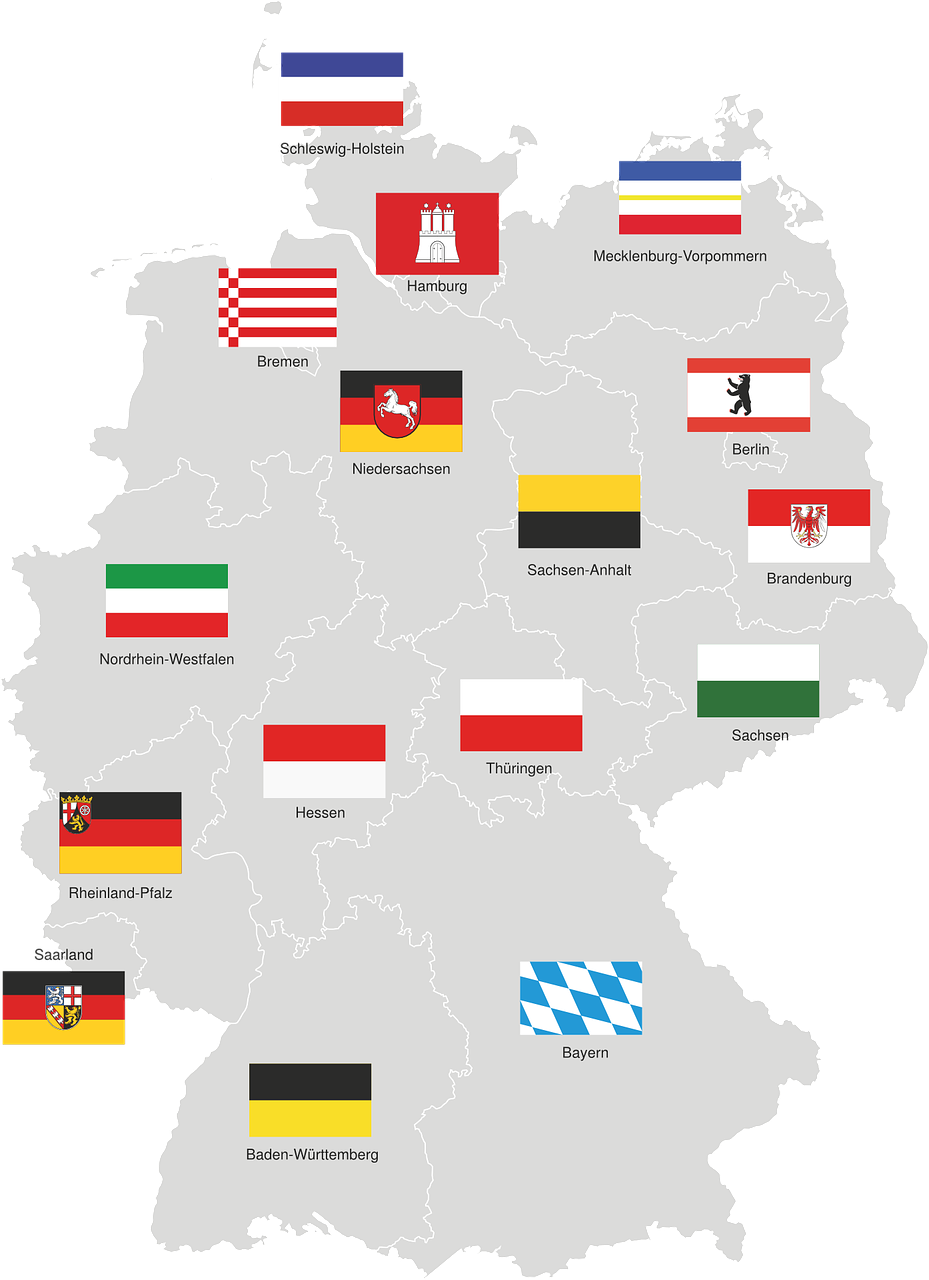
\includegraphics[width=\linewidth]{figures/landkarte.png}
\end{column}

\begin{column}{0.7\textwidth}
In Baden-Württemberg sprechen 40\,\% der Einwohner*innen \textbf{Schwäbisch},
im Rest Deutschlands nur 1\,\%. Baden-Württemberg stellt 13\,\% der
gesamten Einwohnerzahl Deutschlands.

\vspace{0.6em}
\textbf{a)} Berechnen Sie mit dem Satz von Bayes die Wahrscheinlichkeit,
dass eine zufällig ausgewählte Person, die schwäbisch schwätzt, aus
\textbf{Baden-Württemberg} kommt.

\vspace{0.4em}
\textbf{b)} Wie wahrscheinlich ist es, dass diese Person \textbf{außerhalb}
von Baden-Württemberg lebt?
\end{column}
\end{columns}
}
\end{frame}

\begin{frame}[plain]
\end{frame}
\begin{frame}[plain]
\end{frame}

\begin{frame}{Lösung: Satz von Bayes}
\footnotesize
\begin{columns}[T,onlytextwidth]

%----------------- Linke Spalte ------------------
\begin{column}{0.60\textwidth}
\textbf{Gegebene Größen}

\[
\begin{aligned}
p(\text{BW}) &= 0{,}13 & p(\overline{\text{BW}}) &= 0{,}87\\
p(S \mid \text{BW}) &= 0{,}40 & p(S \mid \overline{\text{BW}}) &= 0{,}01
\end{aligned}
\]

\vspace{0.4em}
\textbf{Totale Wahrscheinlichkeit} für „schwäbisch" ($S$):
\[
p(S) = p(S \mid \text{BW})\,p(\text{BW})
     + p(S \mid \overline{\text{BW}})\,p(\overline{\text{BW}})
\]
\[
p(S) = 0{,}40 \cdot 0{,}13 + 0{,}01 \cdot 0{,}87
     = 0{,}052 + 0{,}0087 = 0{,}0607
\]
\end{column}

%----------------- Rechte Spalte ------------------
\begin{column}{0.40\textwidth}
\textbf{a) Satz von Bayes}

\[
p(\text{BW} \mid S) = \frac{p(S \mid \text{BW})\,p(\text{BW})}{p(S)}
\]
\[
p(\text{BW} \mid S) = \frac{0{,}052}{0{,}0607}
                    = \frac{520}{607} \approx 0{,}857
\]
\[
\boxed{p(\text{BW} \mid S) \approx 85{,}7\,\%}
\]

\vspace{0.4em}
\textbf{b) Gegenwahrscheinlichkeit}

\[
p(\overline{\text{BW}} \mid S) = 1 - p(\text{BW} \mid S)
\]
\[
\boxed{p(\overline{\text{BW}} \mid S) \approx 14{,}3\,\%}
\]
\end{column}

\end{columns}
\end{frame}
}

\makequizpage{\QUIZURL}{\QUIZQRCODE}{\QUIZIMAGE}
\makequestionspage{\FRAGENIMAGE}




\makequestionspage{\FRAGENIMAGE}